\section{Reviewer 3}

\subsection{Question 1}
\begin{reviewcomment}
The performance model is unvalidated. This is the central weakness.

FluxArch is evaluated in gem5, with McPAT and CACTI for power and area. The cores derive from real ARM in-order cores, which helps. The full system does not. A 1,024-core design with a custom dataflow engine, a tree interconnect, and a NUMA chiplet hierarchy is never checked against silicon, RTL, or an existing many-core platform. The only error bar in the paper (30\%) covers the technology-node power projection, not the timing model. Every performance and efficiency number depends on this uncalibrated model. The 6.83$\times$ speedup cannot be assessed without validation evidence.
\end{reviewcomment}
We sincerely thank you for your helpful and constructive suggestion. We agree that the performance claims require explicit validation evidence and a clear statement of what remains simulation-based. We therefore address the Engine, core/cache path, and complete system separately.

\begin{enumerate}[label=(\arabic*)]
\setlength{\emergencystretch}{1em}
\item \textbf{RTL-derived Engine timing.} The Engine is a deterministic dataflow implementation whose latency depends on the nuclide count ($N_N$) and reaction-channel count per nuclide ($N_C$) rather than on operand values. We added an RTL-to-gem5 derivation using the fixed operator latencies and the dependencies among the five stages. This produces the closed-form computation latency $12N_NN_C+10N_N+4N_C+3$, which gem5 implements directly instead of fitting an empirical delay.

\revisionlocation{The deterministic Engine timing expression and its RTL derivation are explained in \textbf{Section 4.2}.}

\par\noindent\begin{minipage}{\linewidth}
\excerptlabel{Figure~9 (page 9):}\par
% Manuscript: Figure 9
\begin{figure}[H]
  \centering
  \fbox{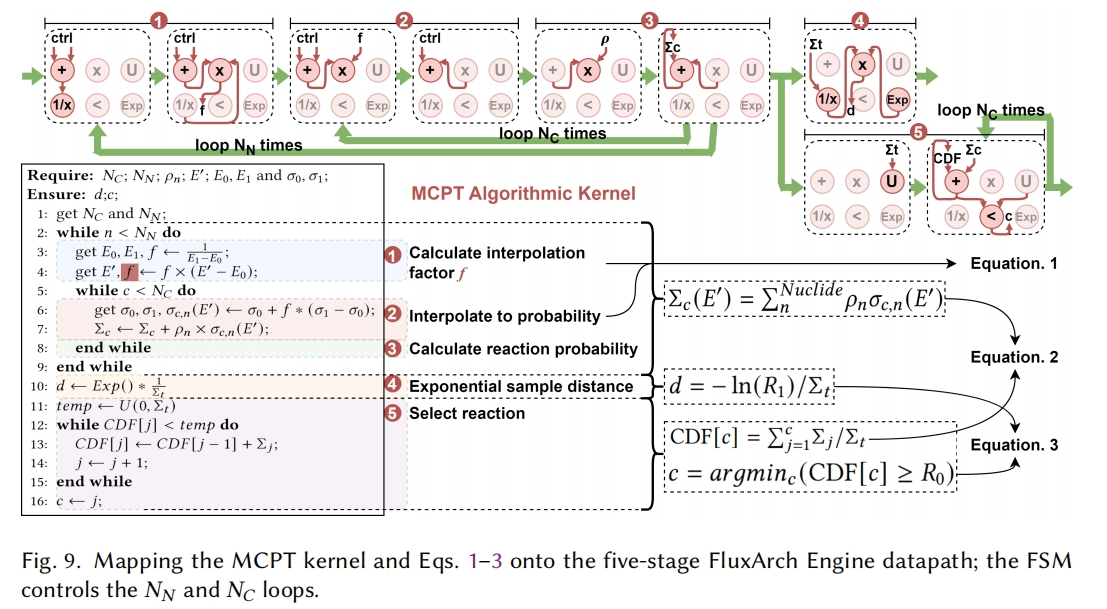
\includegraphics[width=0.9\textwidth]{figures/fig9.png}}
\end{figure}
\end{minipage}\par\medskip

\excerptlabel{Added (Section 4.2, pages 9--10):}\par
\begin{manuscriptexcerpt}
\redsentence{Here, $N_N$ denotes the number of nuclides and $N_C$ the number of reaction channels per nuclide; they determine the outer and inner loop bounds, respectively.}

\redsentence{\textbf{Deterministic Timing Model.}} \redsentence{To meet the timing requirements at the same target clock frequency as the \name\ Core, the RTL operators are partitioned into different numbers of pipeline stages.} \redsentence{Table~2(b) lists the fixed RTL operator latencies using the same symbols as Fig.~9.} \redsentence{Under the computation-only boundary used by the Engine model---excluding launch, stage-transition, \texttt{out\_valid}, and CPU/MMIO input-wait cycles---the five stages take 10 cycles for \redone~($+\to1/x\to\times$, $3+4+3$), 12 cycles for \redtwo~and \redthree~combined~($+\to\times\to+\to\times$, $3+3+3+3$), 7 cycles for \redfour~($1/x\to\times$, $4+3$), and $3+4N_C$ cycles for \redfive~($U\to\{+\to<\}^{N_C}$, $3+N_C(3+1)$).} \redsentence{The resulting latency is
\[
\begin{array}{rl}
L_{\mathrm{Engine}}(N_N,N_C)
&=N_N(10+12N_C)+\max(7,3+4N_C) \\
&=12N_NN_C+10N_N+4N_C+3.
\end{array}
\]} \redsentence{It depends only on the programmed nuclide and reaction-channel counts, not on the numerical operand values.} \redsentence{The gem5 Engine timing directly implements this RTL-derived expression rather than an empirically fitted latency.}
\end{manuscriptexcerpt}

\par\noindent\begin{minipage}{\linewidth}
\revisionlocation{The operator latencies and five-stage timing parameters are specified in \textbf{Table~2(b)}.}

\excerptlabel{Added (Table~2, page 10):}\par
% Revised manuscript: Table 2
\begin{figure}[H]
  \centering
  \fbox{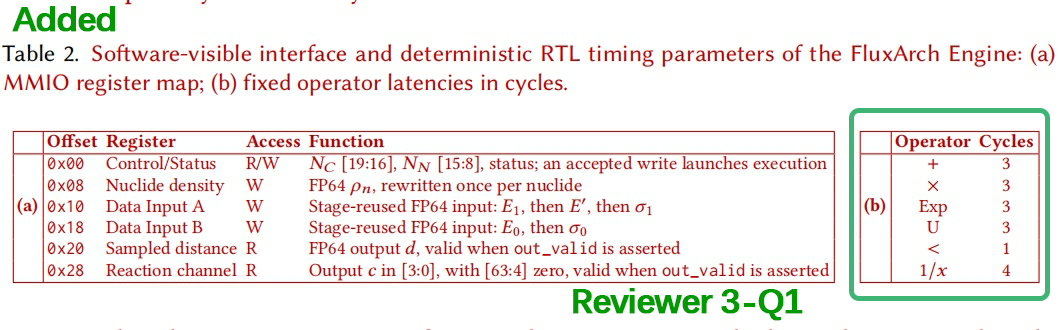
\includegraphics[width=0.9\textwidth]{news/R3-Q1-tab2b.png}}
\end{figure}
\end{minipage}\par\medskip

\item \textbf{Silicon-based core and memory calibration.} The in-order core and cache/DRAM paths are anchored to a Cortex-A53-class silicon reference. We now report the details of six matched native/simulated configurations spanning integer execution, branch control, and dependent random accesses from 16 KiB to 64 MiB. All checksums match, while the measured latency differences yield 6.7\% mean absolute percentage error and 13.5\% maximum absolute percentage error.

\revisionlocation{The silicon-based core and memory calibration protocol, accuracy, and scope are described in \textbf{Section 6.1}.}

\excerptlabel{Added (Section 6.1, page 13):}\par
\begin{manuscriptexcerpt}
\redsentence{\textbf{Core Timing Calibration}.} \redsentence{We calibrate the 2-GHz in-order \name\ Core model against a 2-GB KickPi K3B with a 22-nm quad-core RK3562 Cortex-A53~\papercite{kickpi-k3b,rockchip-rk3562}.} \redsentence{The native process is pinned to one 2-GHz core under stable thermal conditions; both platforms use identical source, GCC 13.3, \texttt{-O2 -fno-tree-vectorize}, seed, warm-up, and timed region.} \redsentence{All six checksums match.} \redsentence{Table~3 reports latency and signed error $100(T_{\rm gem5}-T_{\rm K3B})/T_{\rm K3B}$; across the six tests, the mean and maximum absolute percentage errors are 6.7\% and 13.5\%, respectively.} \redsentence{FluxArch's absolute throughput and speedups are obtained directly from the calibrated simulations.}
\end{manuscriptexcerpt}
\begin{excerptreferences}
\paperreference{rockchip-rk3562}
\paperreference{kickpi-k3b}
\end{excerptreferences}
\par\noindent\begin{minipage}{\linewidth}
\revisionlocation{The six matched RK3562 calibration cases and their latency errors are reported in \textbf{Table~3}.}

\excerptlabel{Added (Table~3, page 13):}\par
% Revised manuscript: Table 3
\begin{figure}[H]
  \centering
  \fbox{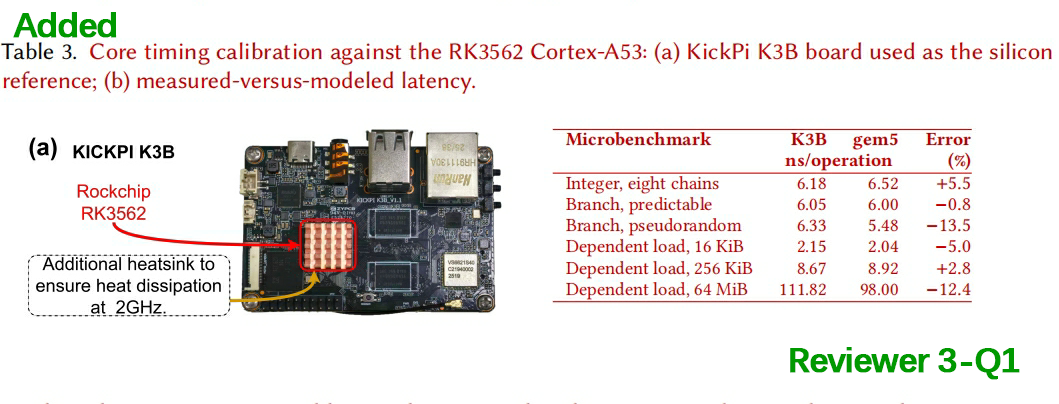
\includegraphics[width=0.9\textwidth]{news/R3-Q1-tab3.png}}
\end{figure}
\end{minipage}\par\medskip



\item \textbf{Performance with the calibrated model.} The performance results reported in \textbf{Section~\ref{subsec:performance_and_power}} and \textbf{Fig.~\ref{fig:perfandpower}(a,b)} already use the calibrated model described above; this revision makes the calibration and RTL timing details explicit. The table below summarizes \name's speedup relative to each evaluated platform with workload orchestration. Each entry is the ratio of \name\ throughput to the platform throughput for the same workload; the final column is the geometric mean of the five ratios.

\par\medskip\noindent\begin{minipage}{\linewidth}
\centering
\small
\textbf{\name\ speedup relative to each platform ($\times$).}\par\smallskip
\setlength{\tabcolsep}{2.5pt}
\begin{tabular}{lrrrrrr}
\hline
\textbf{Platform} & \textbf{CORAL2-P1} & \textbf{CORAL2-P2} & \textbf{CTS2} & \textbf{Homogeneous} & \textbf{XSBench} & \textbf{Geo. mean} \\
\hline
\intel  & 2.05 & 2.33 & 2.13 & 2.42 & 20.98 & \textbf{3.49} \\
\amd    & 0.65 & 0.67 & 0.63 & 0.76 & 5.44 & \textbf{1.02} \\
\ft     & 4.00 & 5.34 & 4.02 & 5.22 & 33.20 & \textbf{6.83} \\
\ampare & 1.93 & 5.38 & 2.57 & 4.16 & 1.45 & \textbf{2.76} \\
\hopper & 1.55 & 3.89 & 2.14 & 2.85 & 1.00 & \textbf{2.06} \\
\hline
\end{tabular}
\end{minipage}\par\medskip

In particular, the 6.83$\times$ figure is the five-workload geometric-mean speedup over FT 64-core, not a uniform speedup across workloads or platforms. These results are supported by silicon-based core/memory calibration and RTL-derived Engine timing.

\end{enumerate}

\subsection{Question 2}
\begin{reviewcomment}
The energy claim excludes DRAM, and the effect is not bounded.

The paper reports large energy-efficiency gains but excludes off-chip DRAM power. MCPT is memory-bound. The paper's own data (Fig. 3(d)(e)) shows the working set exceeds on-chip capacity and forces frequent DRAM access. DRAM energy is therefore likely a large share of system energy. The on-chip scope is disclosed, which is fair. The problem is that the impact is never quantified. A system-level energy result could be materially smaller. As written, the energy advantage is an architectural-efficiency claim, not a system claim, and the gap between the two is unknown.
\end{reviewcomment}
We agree that the original on-chip-only comparison could not support a system-level energy claim for a memory-bound workload. We changed the evaluation to include co-packaged memory through platform telemetry and off-package DDR5 through a common traffic-based DRAMPower model, and we vary the modeled DDR5 component over a $0.5\times$--$2\times$ range to assess sensitivity to missing command-level detail. The conservative process-scaled geometric-mean DRAM-inclusive energy-efficiency advantage remains 1.77$\times$ over H100 and 6.65$\times$ over Intel.

We now explain the choice of the $0.5\times$--$2\times$ range in \textbf{Section 6.1}. Ghose et al.~\papercite{ghose2018vampire} measured DDR3L read currents averaging 54.1\% below datasheet values for one vendor and data-pattern-dependent read-power differences of up to 91.6\%. Shi et al.~\papercite{shi2025drampower} report that DDR4 calibration reduced DRAMPower energy estimates by roughly half for most evaluated SPEC2006 workloads. These results motivate testing sizable modeling discrepancies, but do not establish an error bound for our DDR5 configuration. We therefore select reciprocal factors of 0.5 and 2 to test both overestimation and underestimation, with package power fixed; the range is a sensitivity-analysis choice, not a statistical confidence interval.

For process-scaled energy-efficiency bounds, we independently vary only the scaled FluxArch package power by $\pm30\%$ and each modeled off-package DRAM component over $0.5\times$--$2\times$, while keeping throughput and measured baseline package power fixed. We recompute the performance/W ratio at every endpoint combination and report its minimum and maximum; external DRAM power is not subject to process-node scaling or its 30\% margin.


\revisionlocation{The power-accounting boundary is revised in \textbf{Section 6.1} to include DRAM consistently across platforms.}

\excerptlabel{Revised (Section 6.1, page 14):}\par
\begin{manuscriptexcerpt}
\redsentence{We report DRAM-inclusive system power and energy.} \redsentence{Package power includes cores, caches, NoCs, and integrated memory controllers; for \ft, \ampare, and \hopper, the main memory is co-packaged (DDR4 or HBM) and is consequently covered by platform-level package/device telemetry.} \redsentence{In contrast, the DDR5 DIMMs of \intel\ and \amd, and the DDR5 channels assumed for \name, are physically off-package and are not covered by package-power readings.} \redsentence{We therefore add a separately modeled DRAM component to these platforms, avoiding asymmetric accounting that would include HBM/DDR4 power for the co-packaged-memory platforms but omit DDR5 power for the other platforms.}

\end{manuscriptexcerpt}

\revisionlocation{The traffic-based DRAM model and factor-of-two sensitivity analysis are added in \textbf{Section 6.1}.}

\excerptlabel{Added (Section 6.1, pages 14--15):}\par
\begin{manuscriptexcerpt}
\redsentence{For the DRAM model, we use DRAMPower 5~\papercite{drampower} with DDR5 timing and worst-case current parameters from the JEDEC DDR5 standard~\papercite{jedec_ddr5} and the Micron MT60B2G8HB-48B DDR5-4800 x8 datasheet~\papercite{micron_ddr5}.} \redsentence{\name\ is modeled with 32 single-rank DDR5-4800 channels, each containing eight x8 DRAM devices.} \redsentence{The model includes active-standby background power, refresh power, and read/write transfer power.} \redsentence{The external-memory energy of \intel\ and \amd\ is estimated using the same traffic-based DDR5 model and workload-specific memory traffic.}

\redsentence{Because the simulation does not expose DRAM command traces or row-buffer events, we use a traffic-based DRAM energy estimate rather than claiming command-level precision.} \redsentence{For each \name\ workload, we derive read/write traffic from the memory-system statistics and use the simulated execution time.} \redsentence{Prior DRAM measurement and calibration studies report substantial discrepancies between datasheet-based estimates and measured consumption~\papercite{ghose2018vampire,shi2025drampower}.} \redsentence{Motivated by these findings, we select a $0.5\times$--$2\times$ range for the nominal modeled DRAM power of every off-package DDR5 platform (\intel, \amd, and \name).} \redsentence{This range is a sensitivity-analysis choice, not an empirically established DDR5 error bound or a statistical confidence interval.}
\end{manuscriptexcerpt}
\begin{excerptreferences}
\paperreference{drampower}
\paperreference{jedec_ddr5}
\paperreference{micron_ddr5}
\paperreference{ghose2018vampire}
\paperreference{shi2025drampower}
\end{excerptreferences}

\revisionlocation{The energy-efficiency comparison and conservative lower bounds are updated in \textbf{Section 6.2} to include DRAM power.}

\excerptlabel{Original (Section 6.2, pages 14--15):}\par
\begin{manuscriptexcerpt}
\graysentence{\textbf{Iso-Process Energy Efficiency}.} \graysentence{As shown in Fig.~13(b), the energy efficiency advantage is even more pronounced.} \graysentence{By comparing projected iso-process nodes, we isolate the architectural contributions.} \graysentence{According to Section 6.1, the power projection error is 30\%.} \graysentence{Therefore, we incorporate this margin into our energy efficiency evaluation, which is represented as error bars in our results.}

\graysentence{Without the workload orchestration, the energy efficiency of \name, mainstream server CPUs and high-end GPUs is at odds with each other.} \graysentence{With the orchestration enabled, optimizing data locality and minimizing cross-tile traffic, \name\ demonstrates a superior geometric mean energy efficiency improvement from \textbf{3.98}$\boldsymbol{\times}$ (vs. \ft, 5.69$\times$ discounted by 30\%) to \textbf{9.84}$\boldsymbol{\times}$ (vs. \intel, 14.06$\times$ discounted by 30\%) even accounting for the potential projection error of pessimistic assumption.} \graysentence{We also report the energy efficiency of the raw, unscaled data based on the 22 nm technology node.} \graysentence{Even in this case, \name\ still achieves an energy efficiency improvement of 1.17$\times$ (vs. \hopper) to 4.59$\times$ (vs. \intel).}
\end{manuscriptexcerpt}

\excerptlabel{Revised (Section 6.2, pages 15--16):}\par
\begin{manuscriptexcerpt}
\redsentence{\textbf{DRAM-Inclusive Energy Efficiency}.} \redsentence{Fig.~13(c,d) reports DRAM-inclusive power and energy efficiency under the sensitivity bounds defined in Section~6.1.} \redsentence{Process-scaled results separate architectural effects from process scaling while accounting consistently for external memory.}

\redsentence{In the process-scaled comparison, \name\ improves geometric-mean DRAM-inclusive efficiency by \textbf{2.85}$\boldsymbol{\times}$ over \hopper\ to \textbf{10.58}$\boldsymbol{\times}$ over \intel.}

\redsentence{The sensitivity analysis preserves the process-scaled conclusion: across the combined DRAM and technology-scaling bounds, the geometric-mean improvement with orchestration remains 1.77$\times$ over \hopper\ and 6.65$\times$ over \intel\ at the conservative lower bound.}
\end{manuscriptexcerpt}

\revisionlocation{The energy-efficiency claim is updated in \textbf{Section 9} to reflect the process-scaled, DRAM-inclusive results.}

\excerptlabel{Original (Section 9, page 20):}\par
\begin{manuscriptexcerpt}
\graysentence{We introduced \name, a thousand-core architecture that addresses the performance bottlenecks of MCPT through a large-scale MIMD design and specialized dataflow engines.} \graysentence{By co-optimizing hardware topology and spatial decomposition, \name\ overcomes irregular memory access limitations and delivers geometric mean speedups of up to 1.02$\times$--6.83$\times$ and energy efficiency improvements of up to 3.98$\times$--9.84$\times$ over traditional processors.}
\end{manuscriptexcerpt}

\excerptlabel{Revised (Section 9, page 23):}\par
\begin{manuscriptexcerpt}
\graysentence{We introduced \name, a thousand-core architecture that addresses the performance bottlenecks of MCPT through a large-scale MIMD design and specialized dataflow engines.} \redsentence{It also delivers process-scaled DRAM-inclusive energy-efficiency improvements of 2.85$\times$--10.58$\times$.}
\end{manuscriptexcerpt}

\par\noindent\begin{minipage}{\linewidth}
\revisionlocation{The DRAM-inclusive power and energy-efficiency plots are updated in \textbf{Figure~13(c,d)}. Panel (c) is newly added; panel (d) revises the original energy-efficiency plot.}

\excerptlabel{Revised (Figure~13, page 16):}\par
% Revised manuscript: Figure 13
\begin{figure}[H]
  \centering
  \fbox{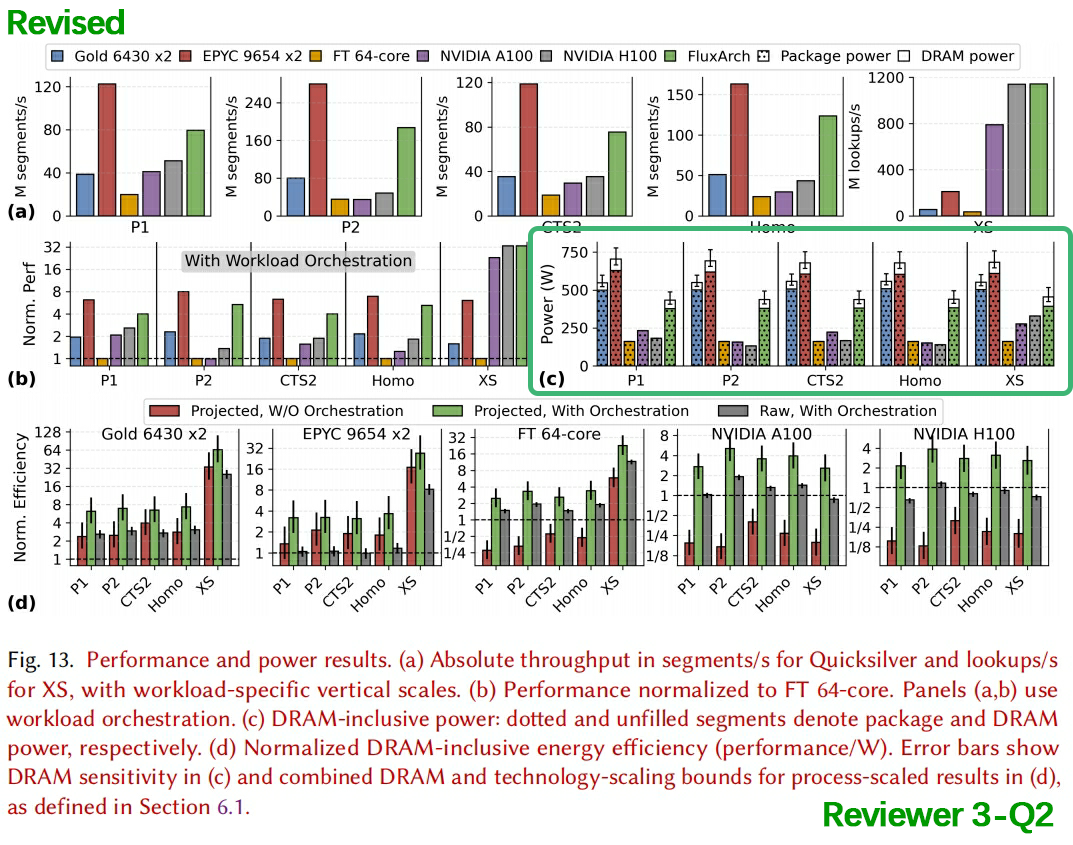
\includegraphics[width=0.9\textwidth]{news/R3-Q2-fig13.png}}
\end{figure}
\end{minipage}\par\medskip

\subsection{Question 3}
\begin{reviewcomment}
The baseline comparison has two specific gaps.

One benchmark (EMCP) is an event-based proxy, and the orchestration is applied to the CPU baselines, so the baselines are not naive. Two gaps remain. Particle-sorting MCPT methods are not evaluated, despite being a known GPU optimization. The comparison against prior specialized MCPT architectures is qualitative only (Table 4); there is no quantitative speedup against those designs. Without these, the claim of superiority over the state of the art is incomplete.
\end{reviewcomment}
We sincerely thank you for your helpful and constructive suggestion. We address the two baseline gaps separately.

\begin{enumerate}[label=(\arabic*)]
\setlength{\emergencystretch}{1em}
\item \textbf{Particle-sorting GPU baseline.} The GPU baseline now includes the particle-sorting optimization rather than comparing only against an unsorted implementation. We evaluated XSBench CUDA variants K4--K6 on both A100 and H100 with sampling, sorting, lookup, and reduction included in the timed and power-measurement interval, and selected the best end-to-end variant, K6. The strengthened H100 baseline reaches 1.140 billion lookups/s, nearly matching \name's 1.143 billion lookups/s; the five-workload geometric-mean speedup of \name\ over H100 is consequently 2.06$\times$.


\revisionlocation{The sorting-enabled GPU baseline selection and end-to-end timing/power boundary are specified in \textbf{Section 6.1}.}

\excerptlabel{Added (Section 6.1, page 14):}\par
\begin{manuscriptexcerpt}
\redsentence{\textbf{GPU Particle-Sorting Baseline}.} \redsentence{For the GPU XSBench baseline, we evaluate the sorting-enabled CUDA variants K4--K6, which group cross-section lookups by material, fuel category, and/or particle energy to reduce warp divergence and improve memory locality.} \redsentence{We use the variant with the highest end-to-end throughput on each GPU; K6, which combines material and energy sorting with material-specific kernels, is the best-performing evaluated variant on both \ampare\ and \hopper.} \redsentence{The reported runtime includes sampling, sorting, cross-section lookup, and result reduction, and the corresponding GPU-board power covers the same execution interval.}
\end{manuscriptexcerpt}

\revisionlocation{The K6 throughput and the resulting comparison with FluxArch are updated in \textbf{Section 6.2}.}

\excerptlabel{Added (Section 6.2, page 15):}\par
\begin{manuscriptexcerpt}
\redsentence{The selected K6 baseline reaches 788.63 million and 1.140 billion XS lookups/s on \ampare\ and \hopper, respectively.} \redsentence{Thus, \name\ and \hopper\ provide nearly identical XS throughput (1.143 versus 1.140 billion lookups/s), while \name's five-workload geometric-mean advantage over \hopper\ is 2.06$\times$.}
\end{manuscriptexcerpt}

\par\noindent\begin{minipage}{\linewidth}
\revisionlocation{The absolute throughput and normalized-performance plots are updated in \textbf{Figure~13(a,b)} using the sorting-enabled GPU baseline. Panel (a) is newly added; panel (b) revises the original normalized-performance plot.}

\excerptlabel{Revised (Figure~13, page 16):}\par
% Revised manuscript: Figure 13
\begin{figure}[H]
  \centering
  \fbox{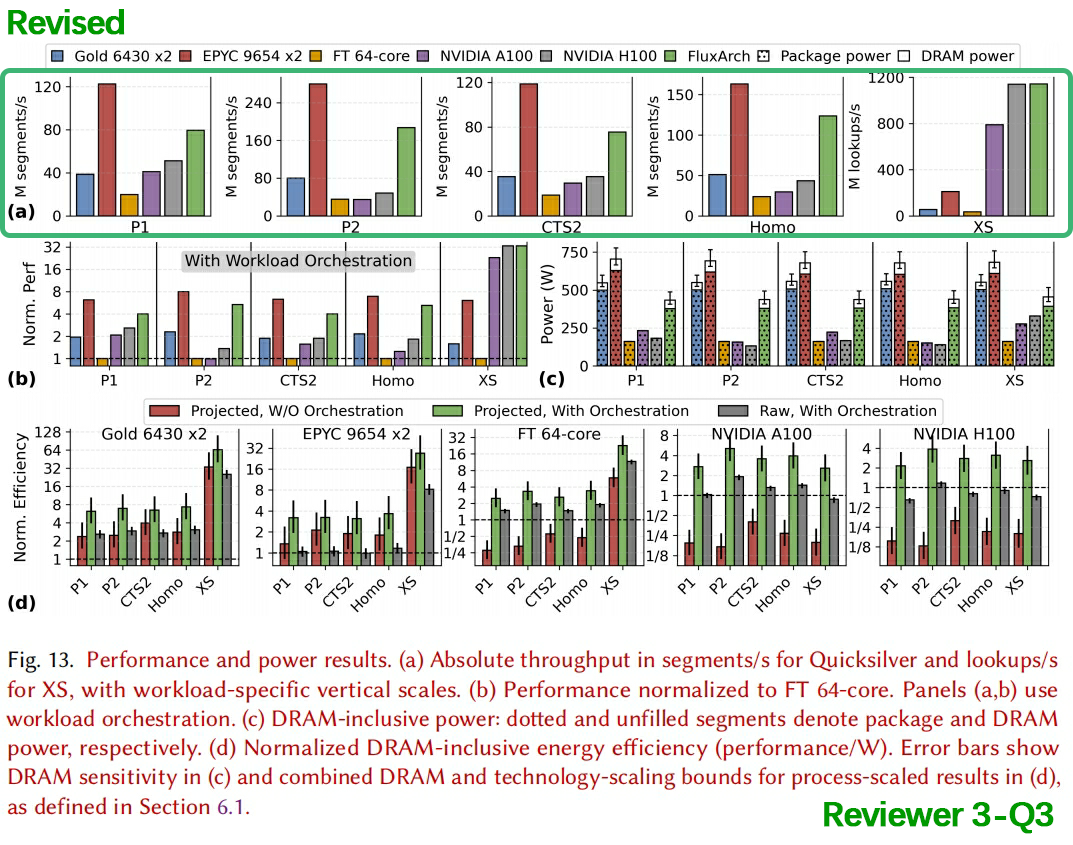
\includegraphics[width=0.9\textwidth]{news/R3-Q3-fig13.png}}
\end{figure}
\end{minipage}\par\medskip

\item \textbf{Prior specialized MCPT architectures.} We added \textbf{Table~7} to compare \name\ with the closely related designs of Fu et al. and Zhang et al., including their core design, hierarchy, cache and memory organization, methodology, workloads, and author-reported quantitative results.

As clarified in \textbf{Section 8}, these results use different workload inputs, resources, baselines, and accounting boundaries. Fu et al.'s ratios are relative to a four-core Cortex-A15 model, whereas Zhang et al.'s scaling efficiency is relative to their own single-core configuration. They therefore cannot be converted into direct speedups over these designs.

A common reimplementation would also require assumptions about implementation and modeling choices not fully specified in the papers. In particular, Zhang et al. do not report a process node or a power/area model. Reconstructing customized simulator configurations and adding such models could make the comparison depend on reconstruction choices as well as architectural differences. We added this limitation to \textbf{Section 8}, rather than presenting assumption-dependent estimates as a validated head-to-head comparison.

\revisionlocation{The comparison with Fu et al. and Zhang et al. is revised in \textbf{Section 8} to clarify the architectural differences.}

\excerptlabel{Original (Section 8, page 19):}\par
\begin{manuscriptexcerpt}
\graysentence{Recent microarchitectural studies have shifted toward specialized, area-efficient designs.} \graysentence{Fu et al. pioneered the use of clustered small cores to improve energy-to-area ratios for MCPT workloads, a foundation subsequently extended by Zhang et al. to a 128-core cluster with optimized parallelization.} \graysentence{Our \name\ system achieves a significant leap forward by: (1) scaling the architecture to 1,024 cores using a hierarchical chiplet-based design; (2) integrating a dedicated execution engine to offload dominant kernels; and (3) proposing a topology-aware hardware-software co-design that transcends the scalability limits of prior clustered small-core architectures.}
\end{manuscriptexcerpt}

\excerptlabel{Revised (Section 8, page 22):}\par
\begin{manuscriptexcerpt}
\redsentence{\textbf{Specialized MCPT Architectures.}} \graysentence{Recent microarchitectural studies have shifted toward specialized, area-efficient designs.} \redsentence{Table~7 compares \name\ with Fu et al.~\papercite{minimctad} and Zhang et al.~\papercite{128mc} in core design, hierarchy, cache and memory organization, evaluation methodology, workloads, and author-reported results.} \redsentence{Fu et al. use simplified in-order cores to improve area and power efficiency, while Zhang et al. scale to 128 cores through 32-core cache-sharing clusters and OpenMP dynamic scheduling.} \redsentence{\name\ combines a 1,024-core hierarchy with a core-local Engine and topology-aware spatial mapping.}

\end{manuscriptexcerpt}
\begin{excerptreferences}
\paperreference{minimctad}
\paperreference{128mc}
\end{excerptreferences}

\revisionlocation{The limits of comparing published results and reconstructing prior designs fairly are added in \textbf{Section 8}.}

\excerptlabel{Added (Section 8, page 22):}\par
\begin{manuscriptexcerpt}
\redsentence{The reported results use substantially different experimental conditions, including workload inputs, core counts, cache and memory configurations, reference baselines, and power-accounting boundaries.} \redsentence{Fu et al. report performance, performance/W, and performance/area relative to a modeled four-core Cortex-A15 system.} \redsentence{Zhang et al. report scaling efficiency relative to their own single-core configuration.} \redsentence{\name's performance and energy-efficiency ratios use the evaluated CPU/GPU platforms as baselines, whereas its scaling efficiency is relative to one core.} \redsentence{Thus, Table~7 places each work's results in context rather than establishing cross-architecture speedups or an efficiency ranking.}

\redsentence{A unified reimplementation would also require resolving implementation and modeling choices not fully specified in the papers, rather than merely matching their listed hardware parameters.} \redsentence{In particular, Zhang et al. do not report a process node or a power/area model.} \redsentence{Reconstructing the customized simulator configurations and supplying missing power/area models would introduce additional assumptions that could affect the results, confounding architectural differences with reconstruction choices and weakening the fairness of a direct comparison.}


\end{manuscriptexcerpt}


\par\noindent\begin{minipage}{\linewidth}
\revisionlocation{The detailed architectural comparison and author-reported quantitative results are added in \textbf{Table~7}.}

\excerptlabel{Added (Table~7, page 22):}\par
% Revised manuscript: Table 7
\begin{figure}[H]
  \centering
  \fbox{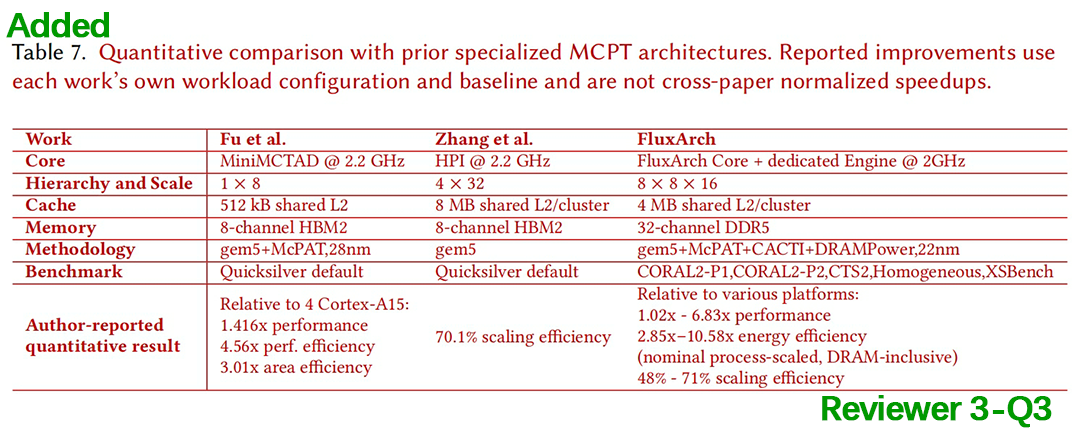
\includegraphics[width=0.9\textwidth]{news/R3-Q3-tab7.png}}
\end{figure}
\end{minipage}\par\medskip

\end{enumerate}
